\chapter{Results}\label{results}

  In this chapter the results of the project will be shown. Annotated screenshots
  of the application will be shown with details of the 
  features and any interaction between components. 

\section{Overview}
\begin{center}
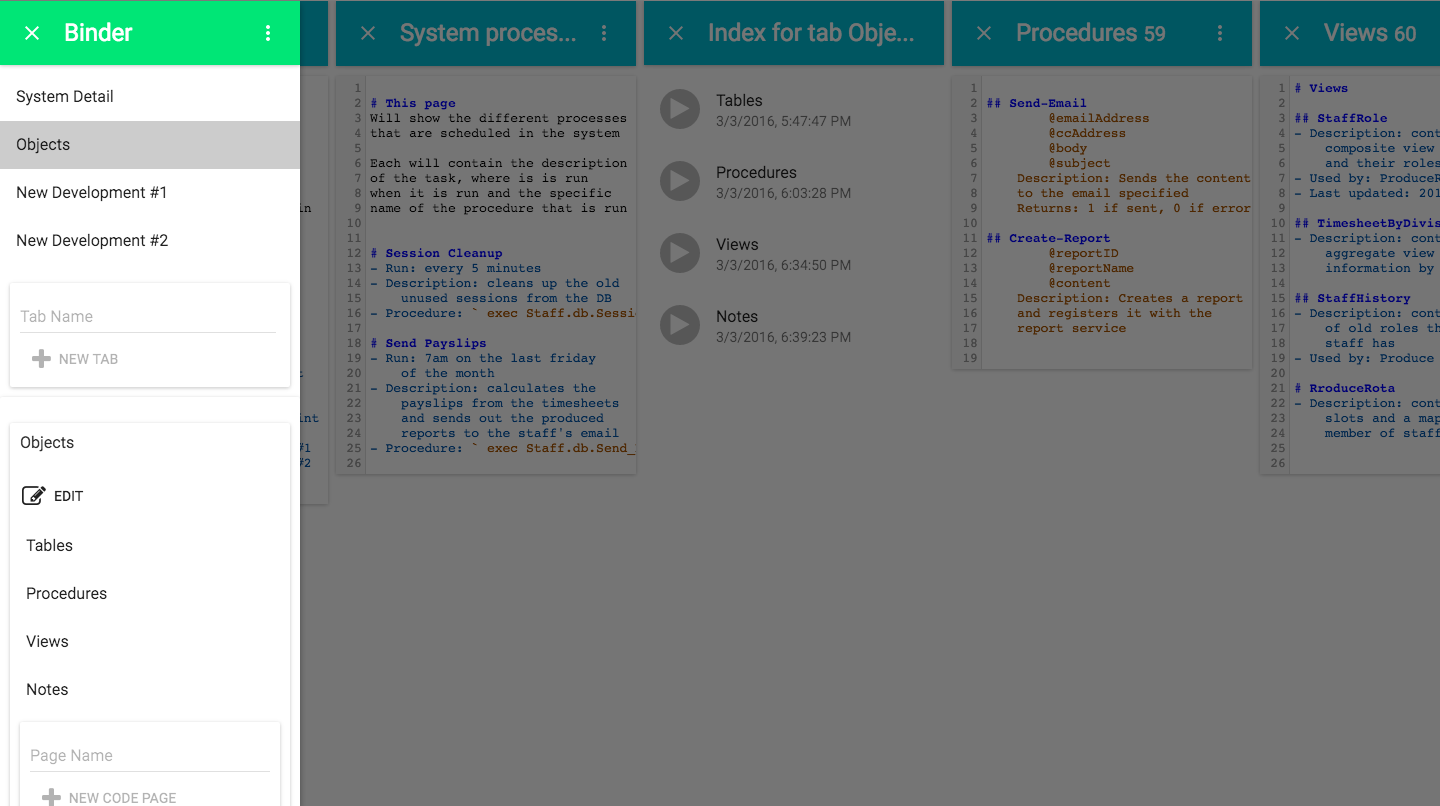
\includegraphics[width=0.8\textwidth]{Figures/Overview.png}
\end{center}

This screenshot shows an open notebook. The left hand side portion of the interface
shows the Binder the main navigational tool. Behind this is the workspace where the open pages
are displayed.

\section{Binder}
The Binder is a navigational interface. It provides a listing for all the files
in the system. The interface is separated into: the Menu bar, where the options are 
displayed, the Tabs list, and the Pages list.

The main purpose is to provide the user with the ability to explore the documents
and offer creation and deletion.

\subsection{Menu}

  \begin{center}
  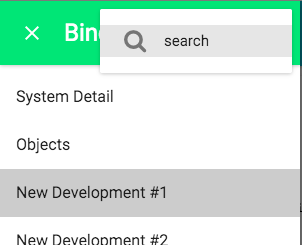
\includegraphics[width=0.3\textwidth]{Figures/Binder-Menu.png}
  \end{center}

  The Menu has only a single ``search'' option, this opens a new search window
  in the workspace.

\subsection{Tabs}

  \begin{center}
  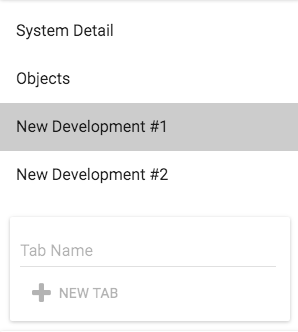
\includegraphics[width=0.3\textwidth]{Figures/Binder-Tabs.png}
  \end{center}

  The Tabs section of the Binder lists the Tabs in the project. Each tab in the
  list can be selected, showing the pages within in the Pages section below.

\subsection{Pages}

  \begin{center}
  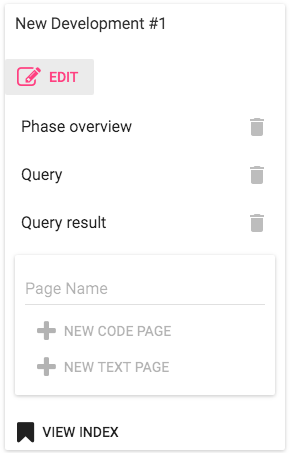
\includegraphics[width=0.3\textwidth]{Figures/Binder-Pages.png}
  \end{center}

  The Pages section is populated when a tab is selected. This section shows
  options for adding new code pages to contain SQL queries and text pages 
  to contain notes. The edit buttion can be selected to toggle edit mode. When
  in edit mode, each page has a delete icon that can be used to remove the page.

  The Index button at the bottom of the section when selected opens an Index page
  for the tab.

\section{Workspace}


  The Workspace is where pages appear when they are opened. The open pages are displayed
  horizontally with new pages opened on the right hand side of old ones. The user can have
  many window open at once.
\subsection{Search}

  \begin{center}
  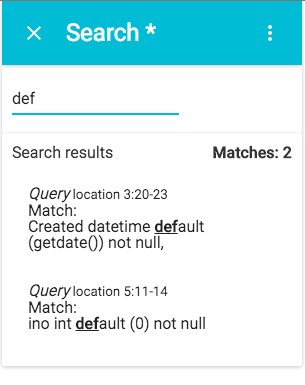
\includegraphics[width=0.3\textwidth]{Figures/Pages-Search.png}
  \end{center}

  The Search page has a single text box for the users search phrase. When the phrase 
  changes, the results in the bottom of the interface update to show the matches.

  Each match has the name of the page, location of the match and the excerpt from 
  the text.

\subsection{Index}

  \begin{center}
  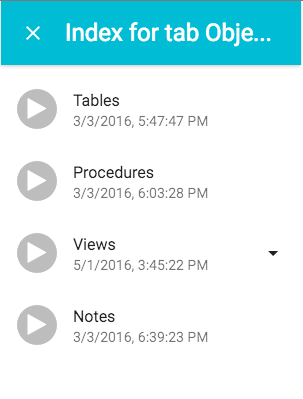
\includegraphics[width=0.3\textwidth]{Figures/Pages-Index.png}
  \end{center}

  The index shows the pages contained within a tab. Each page has the last
  modified date and time next to it from when it was last saved.  

  \begin{center}
  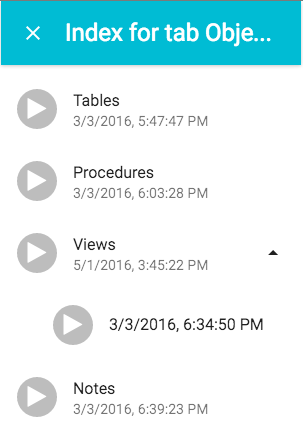
\includegraphics[width=0.3\textwidth]{Figures/Pages-Index2.png}
  \end{center}

  Here one of the pages shown in the index has a previous version stored.

\subsection{Note}

  \begin{center}
  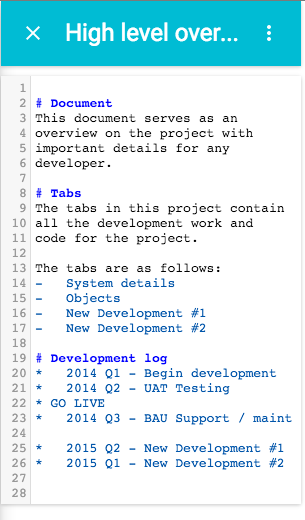
\includegraphics[width=0.3\textwidth]{Figures/Pages-Note.png}
  \end{center}

\subsection{Code}

  \begin{center}
  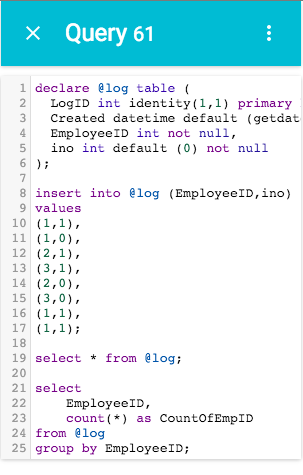
\includegraphics[width=0.3\textwidth]{Figures/Pages-Code.png}
  \end{center}

  \begin{center}
  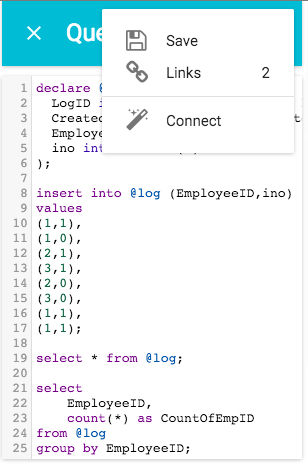
\includegraphics[width=0.3\textwidth]{Figures/Pages-Code-Menu.png}
  \end{center}

  The options available in the menu offer the ability to save, execute and reconnect the page to the database.

  \begin{center}
  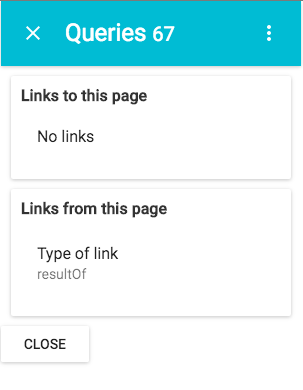
\includegraphics[width=0.3\textwidth]{Figures/Pages-Code-Links.png}
  \end{center}

  The links view, accessed from the menu shows the links this page has to the other items in the
  notebook. 

\subsection{Result}

  \begin{center}
  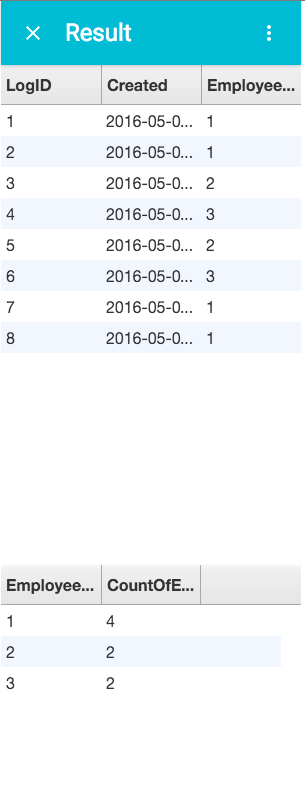
\includegraphics[width=0.3\textwidth]{Figures/Pages-Result.png}
  \end{center}

  The result from a query are shown in a result page. A scrolling table shows the rows in each result set.
  The menu offers the ability to save the result to the notebook for future use.


